\chapter{Implementación}
\label{chap:impl}

Tras realizar el estudio acerca del estado del arte, y basándonos que necesitamos un framework centrado en deep learning que no necesite GPU para ejecutarse, se ha decidido utilizar el lenguaje de programación Python3 con el framework Keras con TensorFlow como back-end.

\bigskip

Cabe destacar que, aunque me hubiera parecido mucho más interesante programar la práctica desde 0, como se proponía en el guión, en lugar de utilizar una librería ya implementada, las restricciones de tiempo y esfuerzo a las que ha tenido que enmarcase esta práctica debido al resto de asignaturas han hecho que finalmente opte por utilizar una framework de desarrollo de aplicaciones \textit{deep learning}.

\section{Framework y librerías utilizadas}

A continuación se presentan los programas más importantes utilizados en esta práctica, así como su versión específica. Se han obviado las dependencias.

\begin{itemize}
  \item \textbf{Python 3.6.6}. Será el lenguaje de programación de la práctica.
  \item \textbf{Keras 2.2.4}. Se utilizará como front-end para trabajar con TensorFlow, ya que actúa como interfaz facilitando su uso.
  \item \textbf{TensorFlow 1.13.0}. Será el corazón de la aplicación
  \item \textbf{Matplotlib 3.0.0}. e utilizará para visualizar el contenido de la base de datos MNIST.
\end{itemize}

\bigskip

\begin{figure}[H]
  \centering
  
\includegraphics[width=0.6\textwidth]{../images/keras-ts}
  \caption{Logos de Keras y TensorFlow}
  \label{fig:logos-keras-ts}
\end{figure}

\bigskip

Para instalar estas librerías usando el proyecto solo es necesario situarse en el directorio raíz y ejecutar \lstinline{make install}.

\section{Detalles comunes de la implementación}

A continuación se presentan la información de la implementación del proyecto. Primero se presentará la información común a todas las versiones del proyecto y a continuación se pasará a describir cada versión por separado. Los resultados detallados de cada versión pueden verse en el capítulo \ref{chap:concl}, mientras que aquí solo se presentará la configuración de cada una.

\bigskip

En total, este proyecto ha pasado por tres versiones, pero es necesario destacar que las versiones no son totalmente sucesivas, sino que entre ellas se realizaron varias subversiones probando diferentes configuraciones de épocas y capas, y no se decidía definir una nueva versión hasta obtener una mejoría suficiente.

\bigskip

Además, se ha utilizado un repositorio en GitHub para realizar el control de versiones de la pŕactica, cuya dirección es \url{https://github.com/gomezportillo/mnist}.

\bigskip

Al final de cada versión se ha publicado una release del proyecto, por lo que las tres versiones pueden verse en la correspondiente sección del repositorio.

\bigskip

Todas las versiones utilizan las mismas librerías, por lo que para probar cualquiera de ellas, y habiendo clonado previamente el repositorio e instalado las dependencias, bastaría con situarse en el directorio raiz y ejecutar \lstinline{git checkout vX.0}, donde  \lstinline{x} es la versión del proyecto, entre 1 y 3, a la que nos queremos mover, y escribir \lstinline{make} para ejecutar la práctica en dicha versión.

\section{Primera versión}

La primera versión fue la más larga y complicada, ya que hubo que configurar todo el entorno de desarrollo para poder trabajar con las librerías elegidas.

\bigskip

En un esfuerzo por hacer los resultados de este proyecto reproducibles, se ha configurado un archivo \lstinline{Makefile} con las instrucciones de instalación necesarias para volver a preparar el mismo entorno de desarrollo. Para instalarlo, simplemente es necesario situarse en el directorio raíz del proyecto y ejecutar \lstinline{make install}, lo que básicamente instalará Python3, luego pip3 y lo usará para instalar las librerías indicadas en el archivo \lstinline{requirements.txt}.

\bigskip

Tras instalar Keras y TensorFlow y sus dependencias fue posible empezar a trabajar en la práctica. Como nunca había trabajado con estas librerías acudí al sitio web de Keras y seguí su tutorial de iniciación\footnote{\url{https://www.tensorflow.org/tutorials/keras/basic_classification}}. En este tutorial se presenta el lenguaje y los principales pasos que hay que seguir para definir y configurar una red neuronal desde cero, así que aunque en el tutorial se utiliza la base de datos \textit{Fashion MNIST}\footnote{\url{https://github.com/zalandoresearch/fashion-mnist}} de prendas de vestir, fue fácil adaptarla para utilizar la base de datos MNIST.

\bigskip

Tras haber configurado el entorno de desarrollo, haber entendido cómo trabajar con  el framework Keras y haber obtenido mis primeros resultados, la configuración final de capas fue la siguiente, usando un modelo secuencial con 15 épocas de entrenamiento.

\bigskip

\begin{itemize}
  \item La primera capa, llamada \textit{Flatten}, transforma  las imágenes de la base de datos de una matriz bidimensional de 28x28 píxeles a un vector unidimensional de 784 píxeles (28*28), lo que permite que la salida sea procesada por capas totalmente conectadas.
  \item La segunda capa, llamada \textit{Dense}, es una capa totalmente conectada con 128 neuronas y una función de activación de rectificación lineal.
  \item La tercera capa, llamada \textit{Dense}, es la capa de salida, con 10 neuronas (una por cada clase) y una función de activación \textit{softmax} para poder realizar predicciones probabilísticas más tarde.
\end{itemize}

\bigskip

La imagen \ref{fig:capas-v1}, generada con la función de Keras \lstinline{plot_model} a partir del modelo, refleja la configuración de capas utilizada.

\bigskip

\begin{figure}[H]
  \centering
  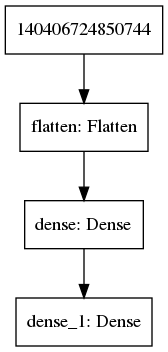
\includegraphics[width=0.3\textwidth]{../images/model-v1}
  \caption{Configuración de capas de la primera versión}
  \label{fig:capas-v1}
\end{figure}

\bigskip

Con esta configuración tan simple pude obtener un porcentaje de acierto sobre el conjunto de entrenamiento del \textbf{99.8\%} y un \textbf{97.62\%} sobre el conjunto de prueba, que me pareció un resultado más que aceptable para una primera versión. Los resultados de esta versión pueden verse detallados en profundidad en el siguiente capítulo.

\bigskip

La ejecución de esta versión duró un poco más que la primera (~300 segundos frente a los solamente ~20 segundos de la primera), así que aunque al principio me planteé usar algún servicio PaaS\footnote{Platform as a Service} como \textit{Amazon Web Services} para ejecutar la práctica, finalmente decidí que debido a su coste y a que los tiempos no eran excesivamente altos podía seguir ejecutándola en mi ordenador personal.

\bigskip

El enlace de esta versión en el repositorio es \url{https://github.com/gomezportillo/mnist/tree/v1.0}.


\section{Segunda versión}

Como ya tenía configurado el entorno de desarrollo y sabía cómo trabajar con el framework elegido, en la segunda versión pude navegar tranquilamente por la API de Keras\footnote{\url{https://keras.io/}} para conocer y entender todas las funciones y parámetros que tiene.

\bigskip

Al final realicé una configuración de 5 capas, usando un modelo secuencial con 15 épocas de entrenamiento.

\bigskip

\begin{itemize}
  \item La primera capa, llamada  \textit{Conv2D}, es una capa convolutiva con la función de activación de rectificación lineal y una ventana convolutiva de 3x3.
  \item La segunda capa, llamada \textit{MaxPooling2D}, es una capa de operación de agrupación máxima con un tamaño de pool de 2x2.
  \item La tercera capa, llamada \textit{Dropout}, descarta el 25\% de las neuronas aleatoriamente para evitar problemas de sobreapendizaje en la fase de entrenamiento.
  \item La cuarta capa, llamada \textit{Flatten}, convierte los datos de entrada de una matriz bidimensional de 28x28 a un vector unidimensional para que puedan ser procesados por capas totalmente conectadas.
  \item La quinta capa, llamada \textit{Dropout}, tiene un número de nodos igual al número de clases del modelo, del 0 al 9, con la función de activación \textit{softmax} para poder realizar predicciones más adelante.
\end{itemize}

\bigskip

La imagen \ref{fig:capas-v2} refleja la configuración de capas utilizada.

\bigskip

\begin{figure}[H]
  \centering
  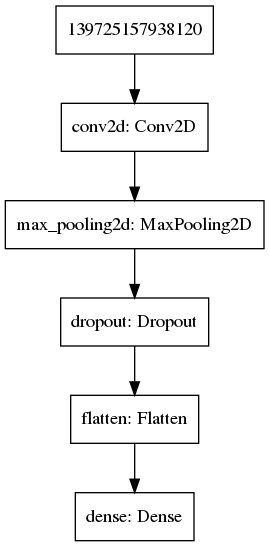
\includegraphics[width=0.45\textwidth]{../images/model-v2}
  \caption{Configuración de capas de la segunda versión}
  \label{fig:capas-v2}
\end{figure}

\bigskip

Con esta configuración, algo más compleja, ya que usa capas convolutivas e intenta evitar el sobreaprendizaje de la red usando funciones dropout, fue posible obtener un porcentaje de acierto sobre el conjunto de entrenamiento de un \textbf{99.27\%} y un \textbf{98.22\%} sobre el conjunto de prueba.

\bigskip

Me pareció interesante que, comparado con la versión anterior, normalmente obtenía resultados algo peores en el conjunto de entrenamiento pero casi un 1\% mejores en el conjunto de prueba, lo que achaqué a que había solucionado los problemas de sobreaprendizaje.

\bigskip

El enlace de esta versión en el repositorio es \url{https://github.com/gomezportillo/mnist/tree/v2.0}.

\section{Tercera versión}

Por último, en la tercera versión del proyecto necesitaba un porcentaje de aciertos lo más cercano al 100\% posible tanto en el conjunto de entrenamiento como en el prueba.

\bigskip

El resultado final fue una configuración de 9 capas, usando un modelo secuencial con 20 épocas de entrenamiento. Como ya había resuelto el problema del sobreaprendizaje pude usar más épocas de entrenamiento que en las versiones anteriores.

\bigskip

\begin{itemize}
  \item La primera capa es una capa convolutiva llamada \textit{Conv2D} con una función de activación de rectificación lineal, 32 mapas característicos y una ventana convolutiva de 4x4.
  \item La segunda capa es una capa convolutiva llamada \textit{Conv2D} con la función de activación de rectificación lineal y una ventana convolutiva de 3x3.
  \item La tercera capa, llamada \textit{MaxPooling2D}, es una capa de operación de agrupación máxima con un tamaño de pool de 2x2.
  \item La cuarta capa, llamada \textit{Dropout}, descarta el 20\% de las neuronas aleatoriamente para evitar problemas de sobreapendizaje en la fase de entrenamiento.
  \item La quinta capa, llamada \textit{Flatten}, convierte los datos de la matriz bidimensional en un vector lineal para que la sexta capa pueda ser una capa completamente conectada.
  \item La sexta capa, llamada \textit{Dense}, es una capa completamente conectada con 248 neuronas y función de activación de rectificación lineal.
  \item La séptima capa, llamada \textit{Dense}, es una capa completamente conectada con 124 neuronas (la mitad que la anterior) y función de activación de rectificación lineal.
  \item La octava capa, llamada \textit{Dropout}, vuelve a descartar el 40\% de las neuronas aleatoriamente.
  \item La novena capa, llamada \textit{Dense}, es la capa de salida, con 10 neuronas (una por cada clase) y una función de activación \textit{softmax} para poder realizar predicciones probabilísticas más adelante.
\end{itemize}

\bigskip

La imagen  \ref{fig:capas-v3} refleja la configuración final de capas utilizada.

\bigskip

\begin{figure}[H]
  \centering
  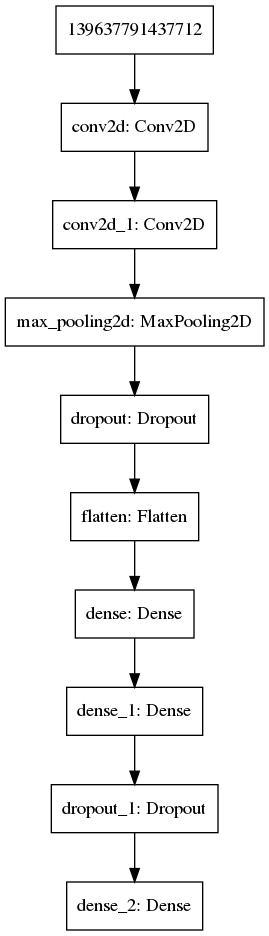
\includegraphics[width=0.5\textwidth]{../images/model-v3}
  \caption{Configuración de capas de la tercera versión}
  \label{fig:capas-v3}
\end{figure}

\bigskip

Con esta configuración pude obtener un porcentaje de aciertos sobre el conjunto de prueba de un \textbf{99.91\%} y un \textbf{99.15\%} sobre el conjunto de prueba.

El enlace de esta versión en el repositorio es \url{https://github.com/gomezportillo/mnist/tree/v3.0}.
